\documentclass[a4paper]{ctexart}

\setmainfont{Microsoft Sans Serif}
\setCJKmainfont{STFangsong}
\usepackage[raggedright]{titlesec}
\usepackage{fancyhdr}
\usepackage{graphicx}
\usepackage{amsmath}
\usepackage{pifont}
\usepackage[perpage,symbol,marginal]{footmisc}
\usepackage{geometry}
\usepackage{graphicx}

\geometry{left=2.54cm,right=2.54cm,top=2.54cm,bottom=2.54cm}

\DefineFNsymbols{circled}{{\ding{192}}{\ding{193}}{\ding{194}}
{\ding{195}}{\ding{196}}{\ding{197}}{\ding{198}}{\ding{199}}{\ding{200}}{\ding{201}}}
\setfnsymbol{circled}

\pagestyle{plain}

\begin{document}

\setcounter{section}{0}
\setlength{\parindent}{0em}
\setlength{\parskip}{1.2ex}

\title{TSP作业报告}
\date{2016年5月24日}
\maketitle

\section{交叉算子}
本算法使用的是实现较为简单和常用的顺序交叉(order cross),即先选取两个交叉点,保留父代A中两个交叉点之间的基因,然后按顺序从父代B中将剩余的基因填到剩下的位置:
\begin{figure}[htbp]
\begin{large}
$$
\begin{aligned}
12\ |\ 345\ |\ 6\\
56\ |\ 231\ |\ 4
\end{aligned}
\quad \Longrightarrow \quad
\begin{aligned}
345\ |\ 621\\
231\ |\ 645
\end{aligned}
$$
\end{large}
\caption{顺序交换算子}
\end{figure}
\par
该算法实现简单,但是没有用到任何启发式的信息,仅仅是随机保留某个父代的一个子串,效率上没有保证。\par
\section{变异算子}
本算法的变异算子带有一定的启发式信息。考虑颠倒基因中的一个子串,对于整个TSP的路径来说只是修改了两条边的连接方式:\par
\begin{figure}[htbp]
\centering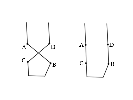
\includegraphics[width=3.5in]{1}
\caption{变异算子}
\end{figure}
这样一来,如果满足不等式:$AB + CD > AC + BD$,那么变异后的结果一定更优。我们这样设计算法:首先随机选取子串的一个端点,枚举第二个端点,找到第一个能满足不等式的点直接颠倒该子串,找不到就不变异。这样一定能保证变异后的结果比原来更优。\par

\section{选择算子}
经过测试,传统的轮盘赌选择方式效果非常差,因为选择和变异后父代直接被舍弃了,导致优的个体反而可能变得更差。这里用的是这样的方法:将子代和父代放在一起,按照适应度从大到小排序(即按照路径长度从小到大排序),然后直接淘汰排名超过种群大小的个体。这种方法可能比较简单,但是收敛比较快。\par
\section{参数设置}
种群大小:$M=200$;$P_c=P_m=1$,即交换和变异一定发生;交换的时候枚举每一个个体为父代$A$,随机选择另一个父代$B$($A\not=B$)。因为父代不会被直接舍弃,因而每次都进行交换和变异。\par
每经过1000代纪录一次数据,每轮训练为10000代,两轮之间最优个体不再改变后终止。除了最大一组数据(bm33708)在运行10小时后还未终止,被手动终止外,其他所有数据都运行结束了。\par
\section{结果}
\begin{table}[htbp]
$$
\begin{array}{|c|c|c|c|c|}
\hline
 \text{测试数据} & \text{路径长度}  & \text{误差} & \text{运行时间} & \text{收敛代数} \\
\hline
\text{dj38} & \text{6659.43} & \text{0.05\%} & \text{6.9s} & \text{20000} \\
\hline
\text{qa194} & \text{9638.7} & \text{3.06\%} & \text{26.5s} & \text{20000} \\
\hline
\text{lu980} & \text{12140.1} & \text{7.05\%} & \text{242.2s} & \text{60000} \\
\hline
\text{mo14185} & \text{472985} & \text{10.67\%} & \text{185min} & \text{120000} \\
\hline
\text{bm33708} & \text{1070720} & \text{11.61\%} & \text{600min} & \text{181000} \\
\hline
\end{array}
$$
\caption{五组测试数据的结果}
\end{table}
\section{总结和改进思路}
假设城市个数为$N$,种群规模为$M$。交换和变异的复杂度都是$O(N)$的,因而运行一代的复杂度为$O(MN)$,由于代数非常大(10000-100000),对于大数据是非常慢的。从记录看,最大的一组数据(bm33708)在终止前产生了181000代,而第二大的数据(mo14185)产生了120000代,但运行时间差了3-4倍左右。\par
从记录看,该算法收敛速度呈指数级递减,最终稳定在某个和答案较为接近的值;从图像看,最终的答案图像虽然和标准解答非常相似,但是有很多地方整体上是非常不同的,需要做较大的改变才能变得更优,这说明收敛到了一个局部最优解。降低种群规模不会影响收敛速度(运行速度反而大幅度提高),但是会大大影响最终得到的局部最优解;可以推测提高种群规模能使局部最优解更接近答案。这说明提高种群的多样性有助于得到更加优的答案。得到局部最优解也可能和选择算子相关,可以考虑适当在选择中加入随机性来增加多样性,或者按照模拟退火的思路,种群规模随时间指数级递减。\par
\begin{figure}[htbp]
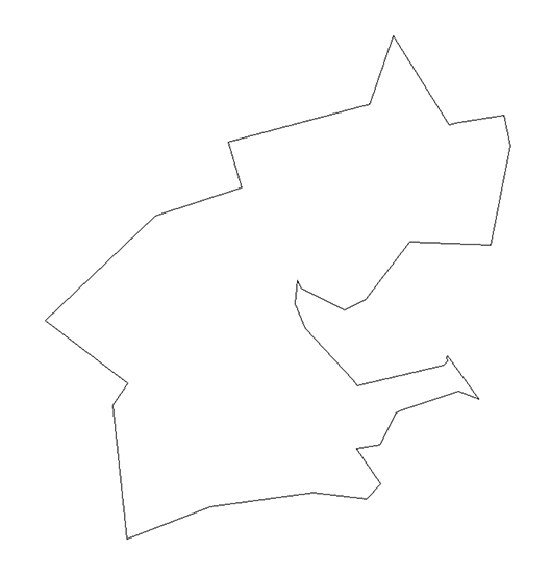
\includegraphics[height=2.65in]{2}
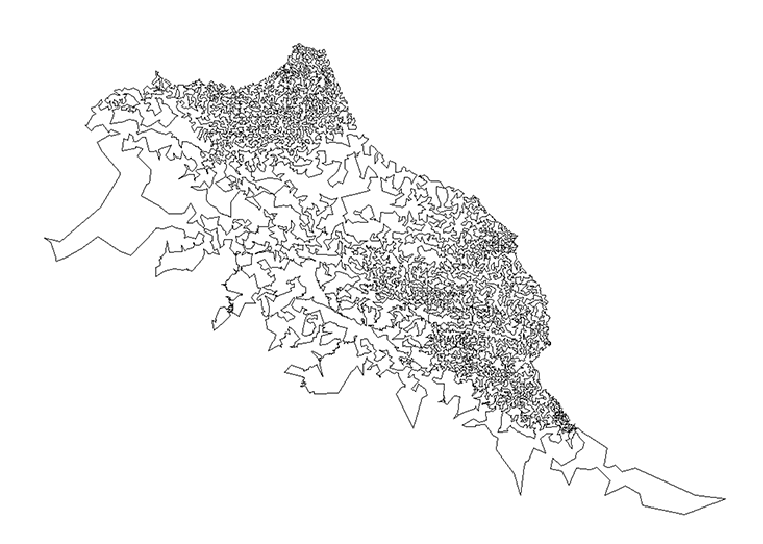
\includegraphics[height=2.65in]{3}
\caption{dj38和mo14185的结果}
\end{figure}
目前初始种群是完全随机的(路径长度约为标准解的50-100倍),需要较长时间才能达到比较好的情况。按照一些同学的思路,实际上可以直接通过贪心等方法构造一组非常优的解(几秒钟构造出来的解甚至优于训练几个小时),再进行训练。\par
\end{document}
